\documentclass[11pt]{article}
\usepackage{amsmath}
\usepackage[utf8]{inputenc}

\usepackage{xcolor}
\usepackage{setspace}
\usepackage{graphicx}
\usepackage[hidelinks,colorlinks=true,linkcolor=blue,citecolor=blue]{hyperref}

\newcommand{\blue}[1]{\textcolor{blue}{#1}}
\newcommand{\red}[1]{\textcolor{red}{#1}}
\newcommand{\link}[1]{\href{#1}{\blue{#1}}}

\definecolor{keywordred}{RGB}{255, 123, 114}
\definecolor{keywordorange}{RGB}{255, 166, 86}
\definecolor{keywordpurple}{RGB}{210, 168, 254}
\definecolor{commentblue}{RGB}{165, 214, 255}
\definecolor{noneblue}{RGB}{121, 192, 255}

\title{Ram Installation Guide}
\author{Will Assad\footnote{Department of Mathematics, University of Toronto} , Ariel Chouminov\footnote{Department of Computer Science, University of Toronto} , Ramya Chawla$^\dag$, Zain Lakhani$^\dag$}
\date{\today}

\begin{document}

\maketitle

\noindent This is a summary of how to use the Ram programming language on MacOS and Windows. The Python script can simply be run with a virtual environment satisfying \texttt{requirements.txt}.

\section{Using MacOS}

\subsection*{Python Console}

    \begin{itemize}
        \item You can write a new \texttt{.ram} file in any text editor. We even defined custom syntax highlighting for \texttt{*.ram} files in PyCharm! 
            
        \begin{center}
            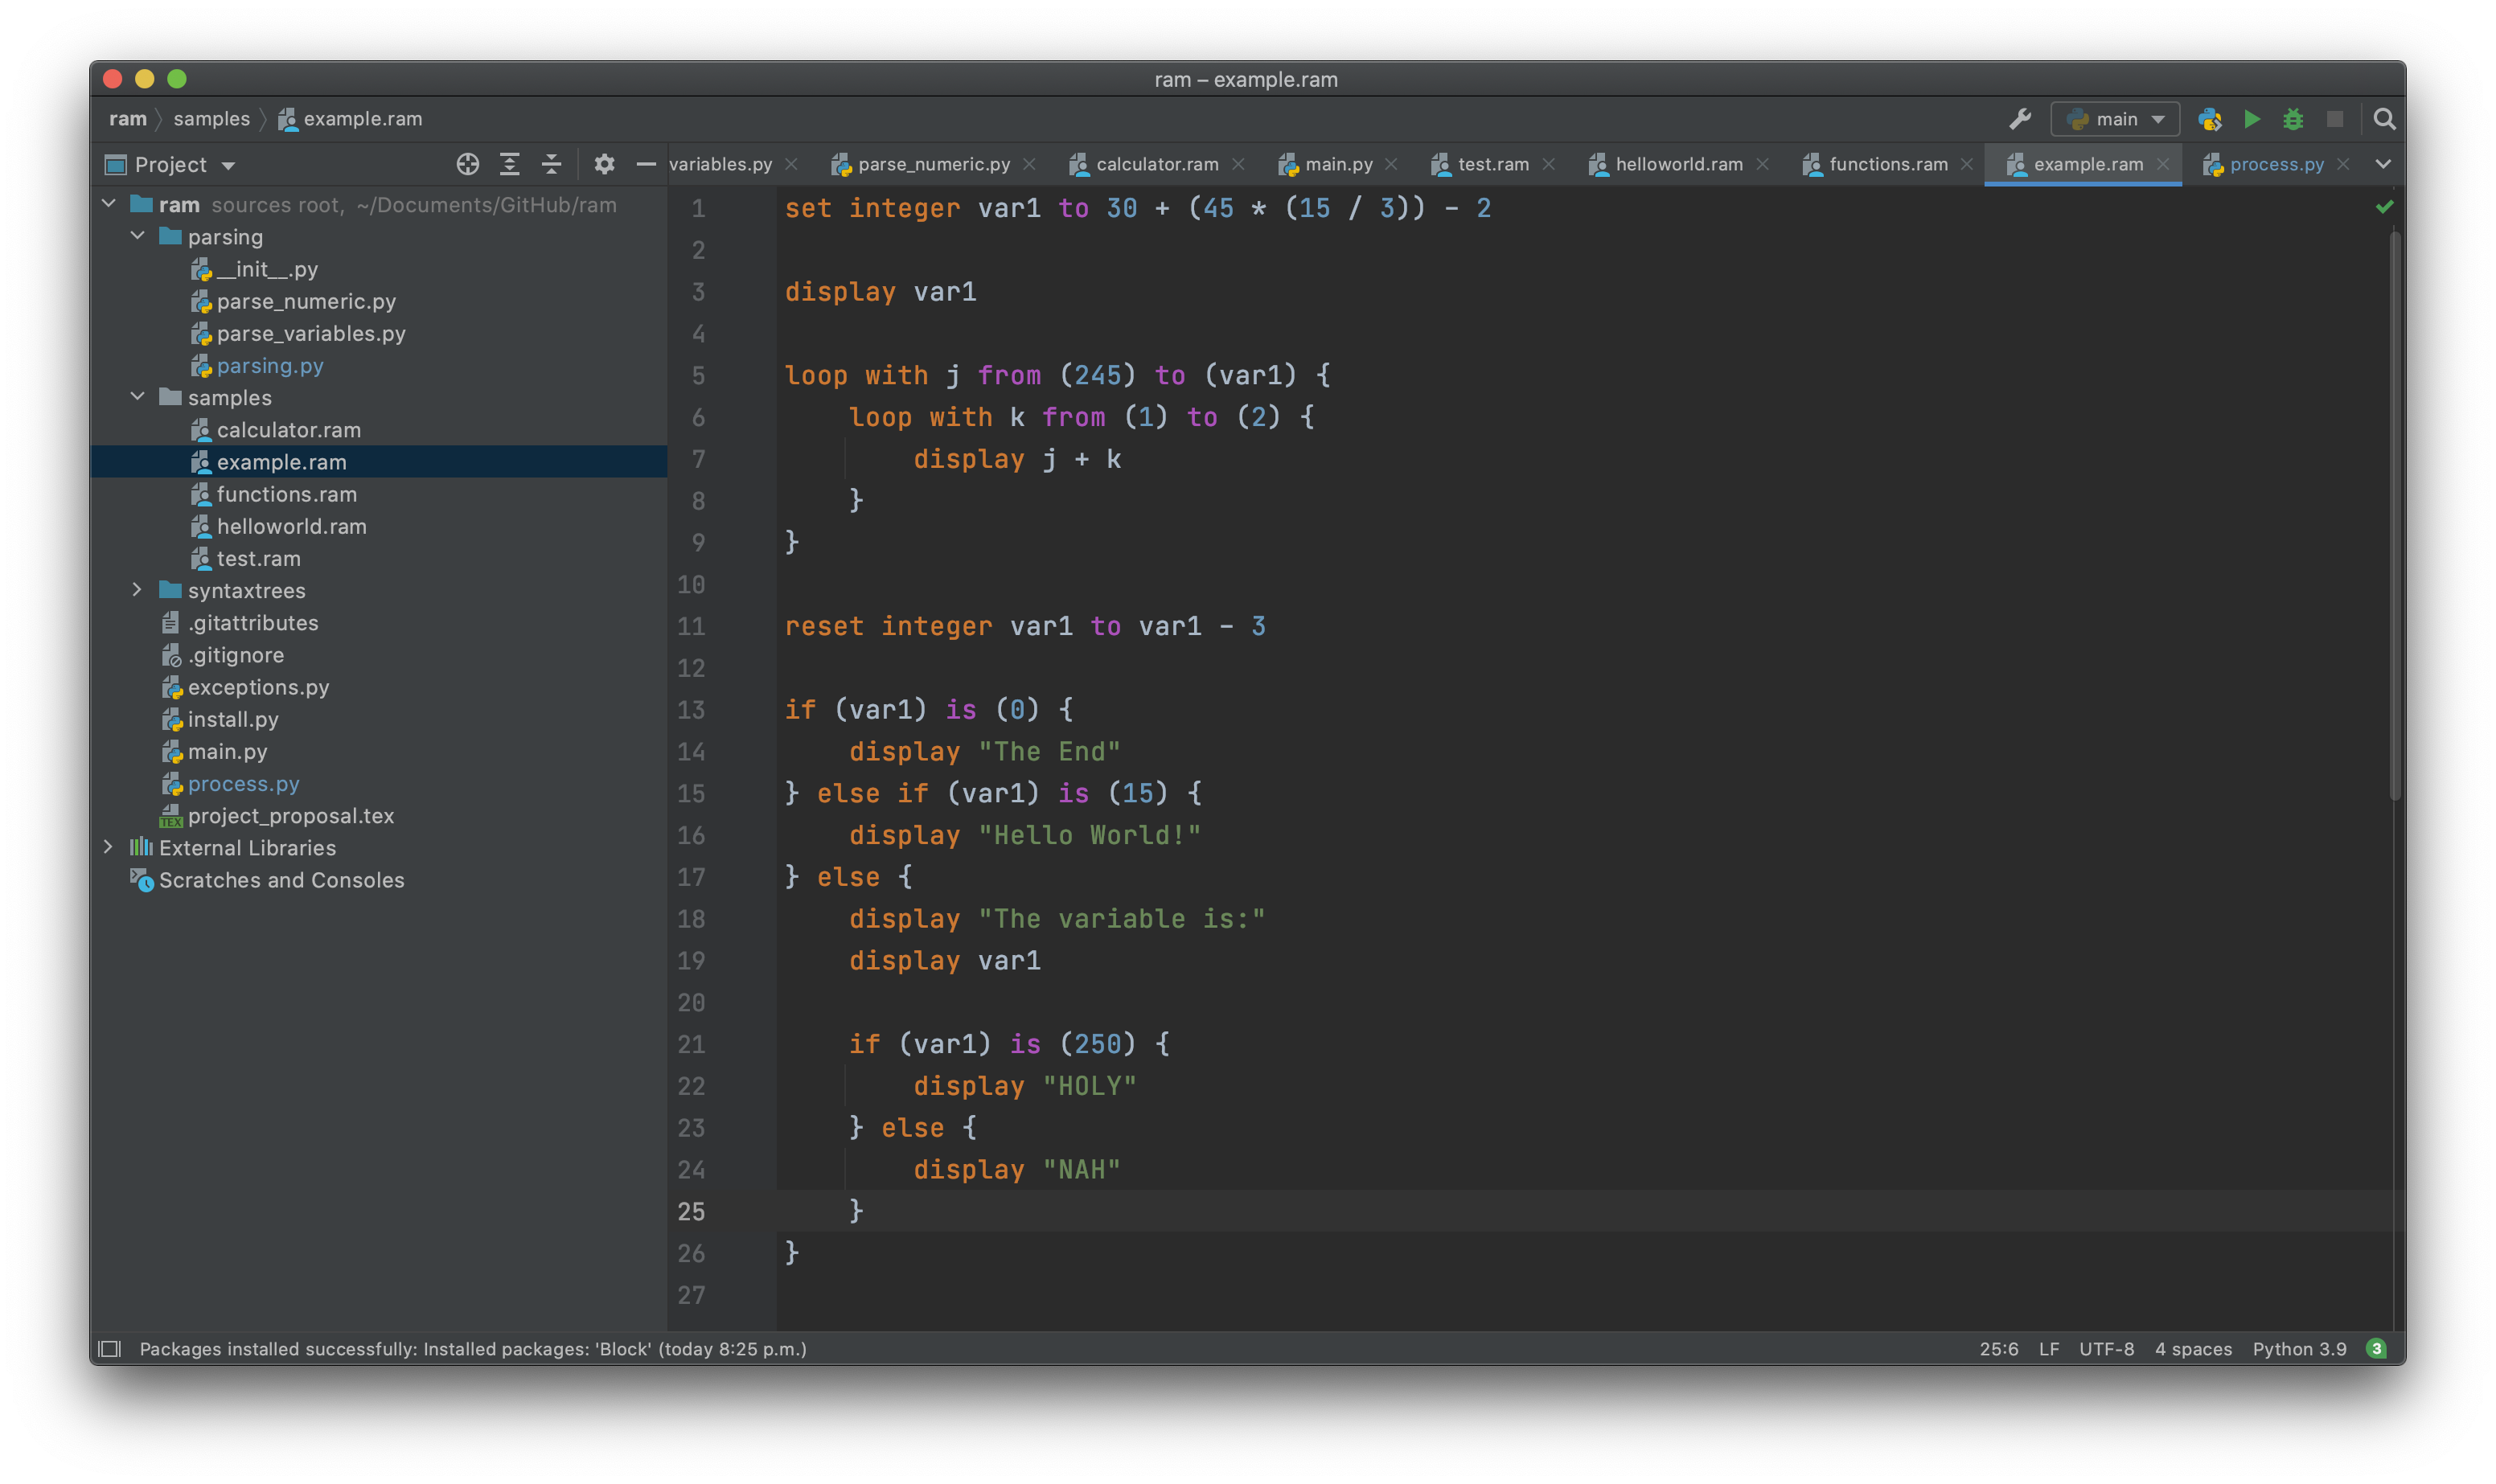
\includegraphics[scale=0.18]{terminal5.png}
        \end{center}
            
        \item Run main.py
            
        \item You will be prompted to enter the file path of the .ram file to run.
            
        \bigskip
            
        \bigskip        
        
        \newpage
        
    \end{itemize}
    
\subsection*{Terminal}
    
    \begin{itemize}
        \item Open Terminal and type \texttt{which python} or \texttt{which python3} (depending on the version installed).
            
        \begin{center}
            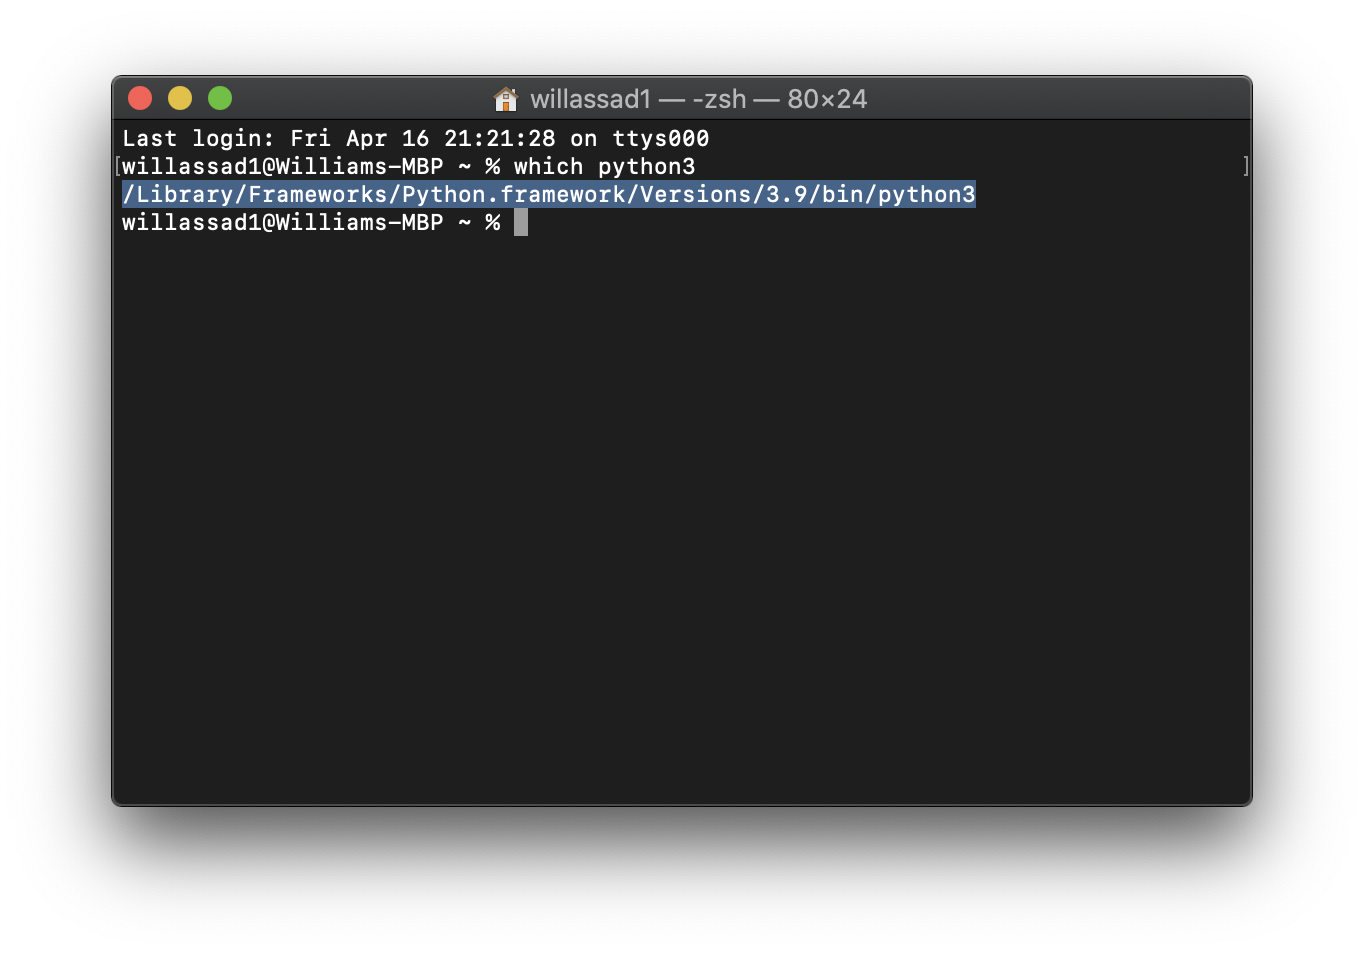
\includegraphics[scale=0.45]{terminal1.png}
        \end{center}
            
        \item Copy the result and then open \texttt{main.py} and paste the result after the \texttt{!\#}.
             
        \begin{center}
            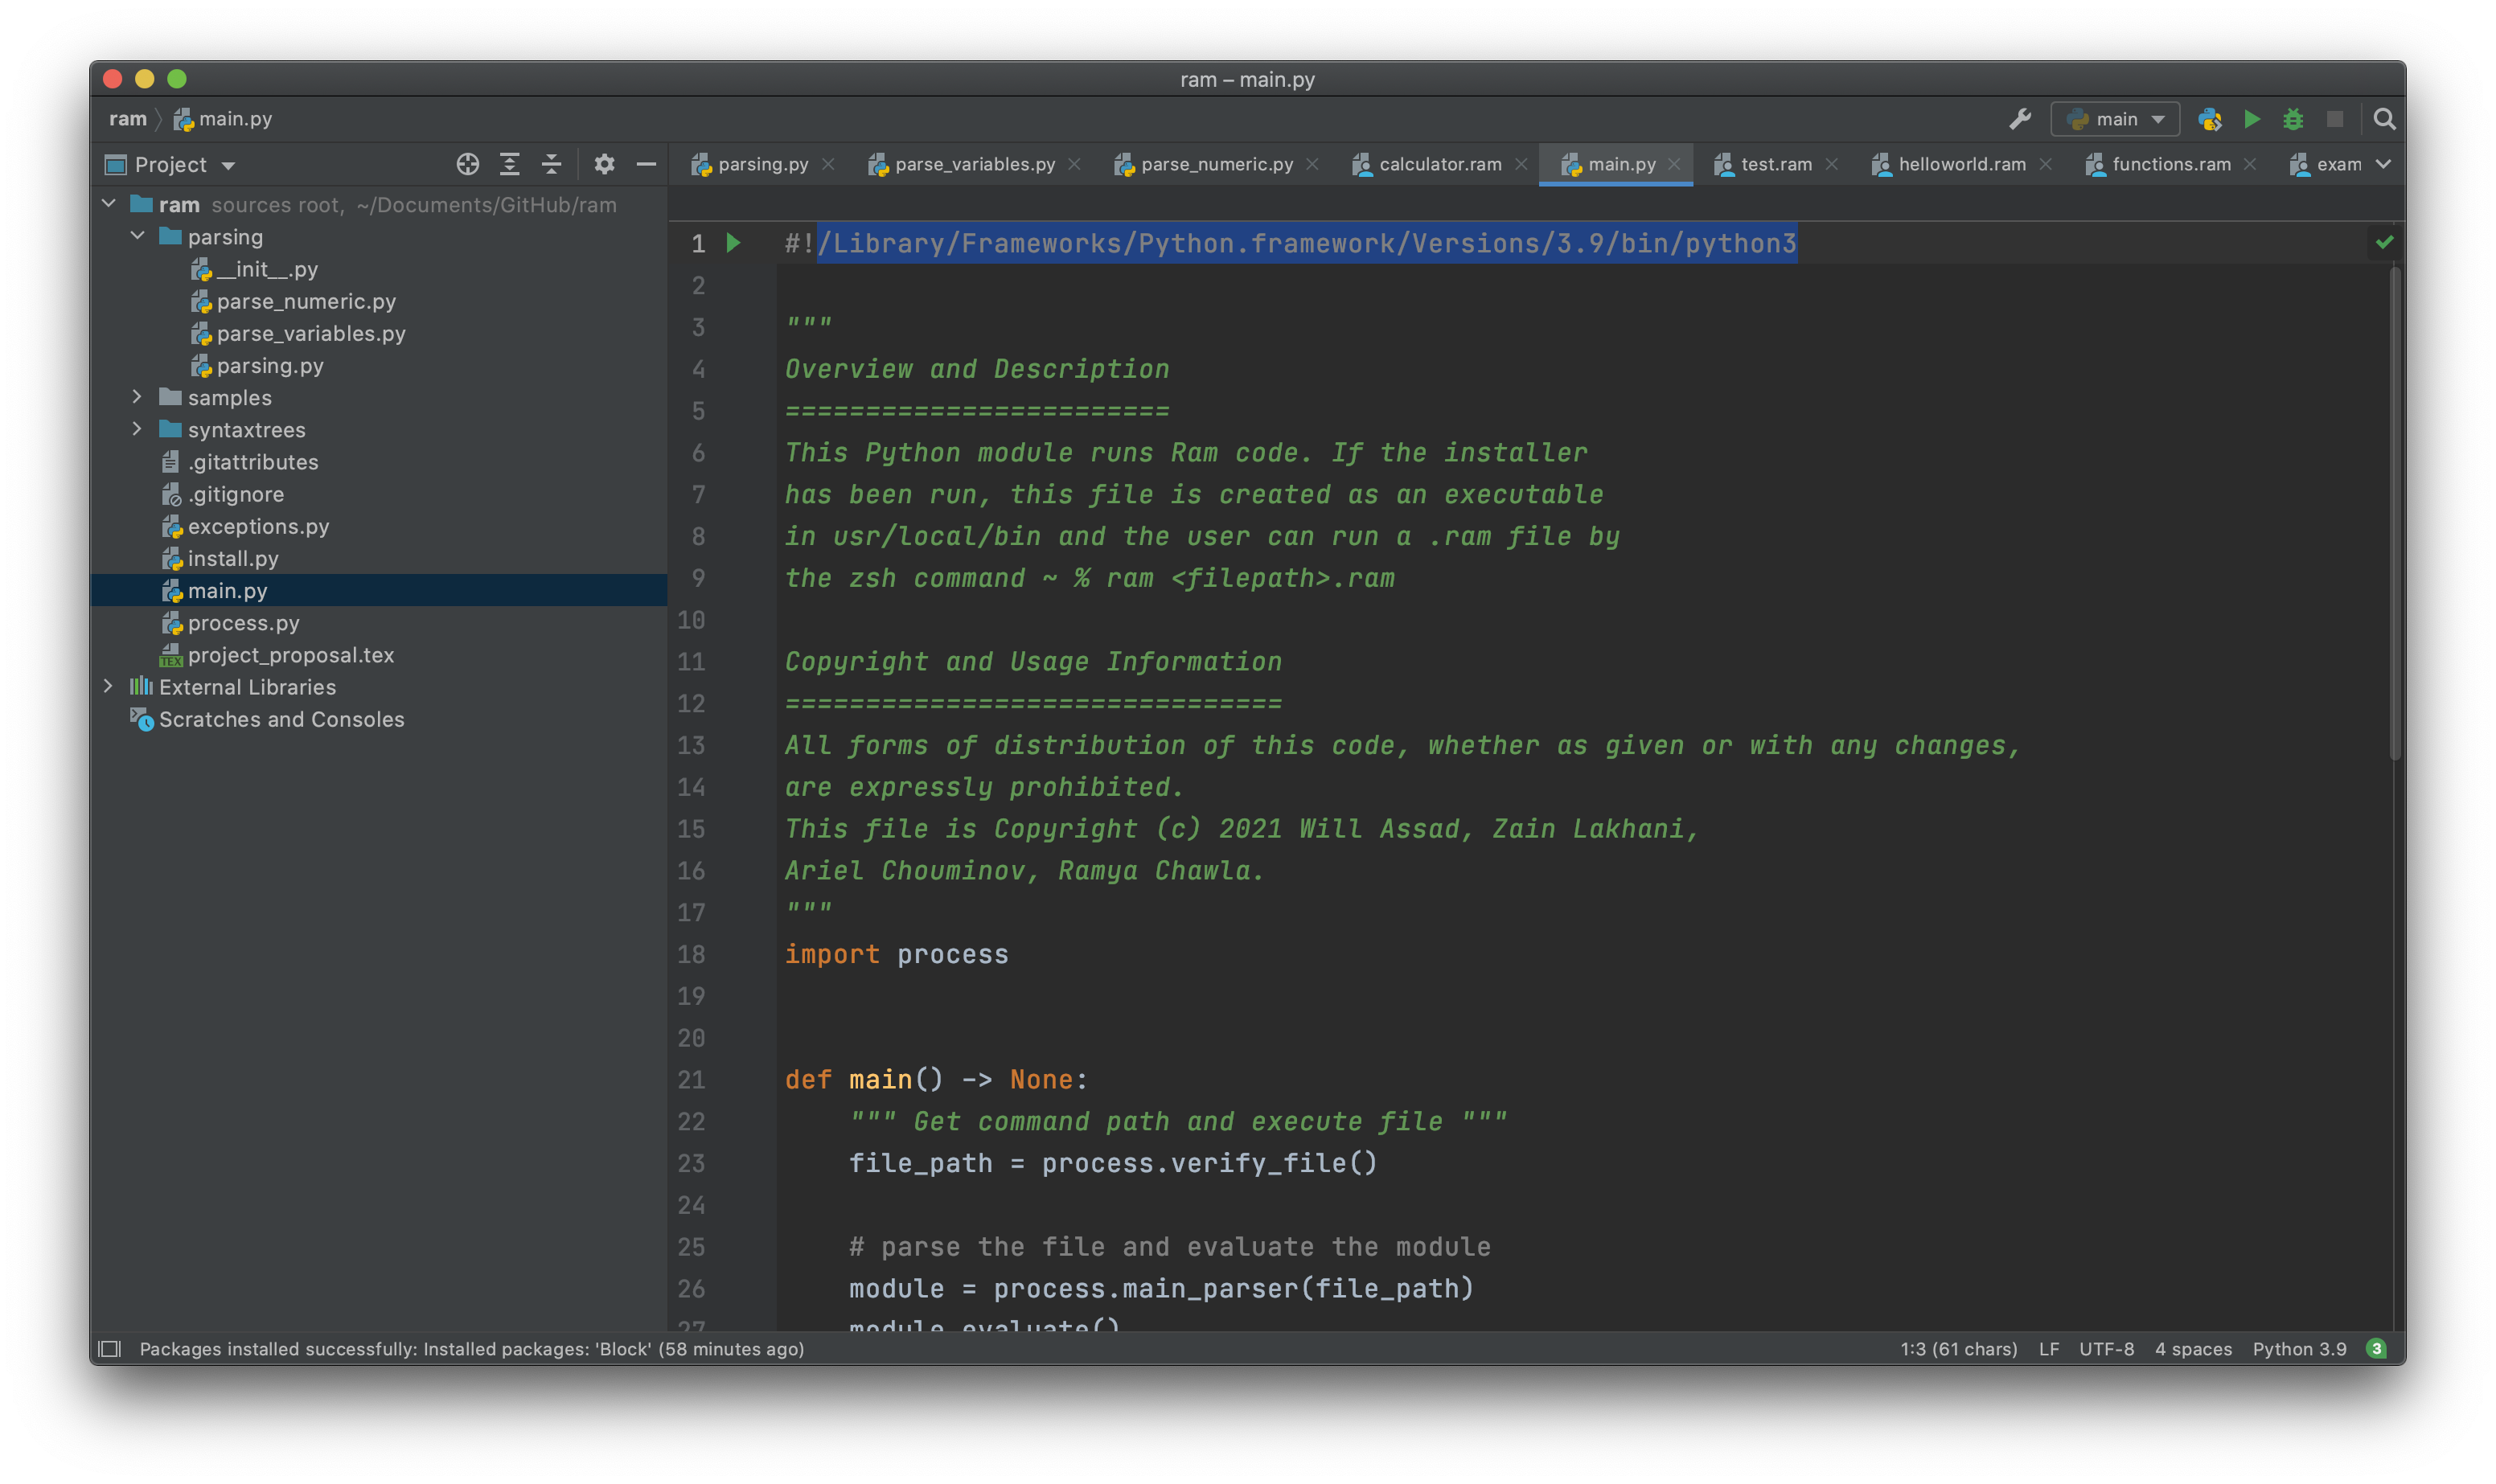
\includegraphics[scale=0.2]{terminal4.png}
        \end{center}
        
        \newpage
            
        \item Navigate to the main \texttt{ram} program directory (wherever stored).
            
        \begin{center}
            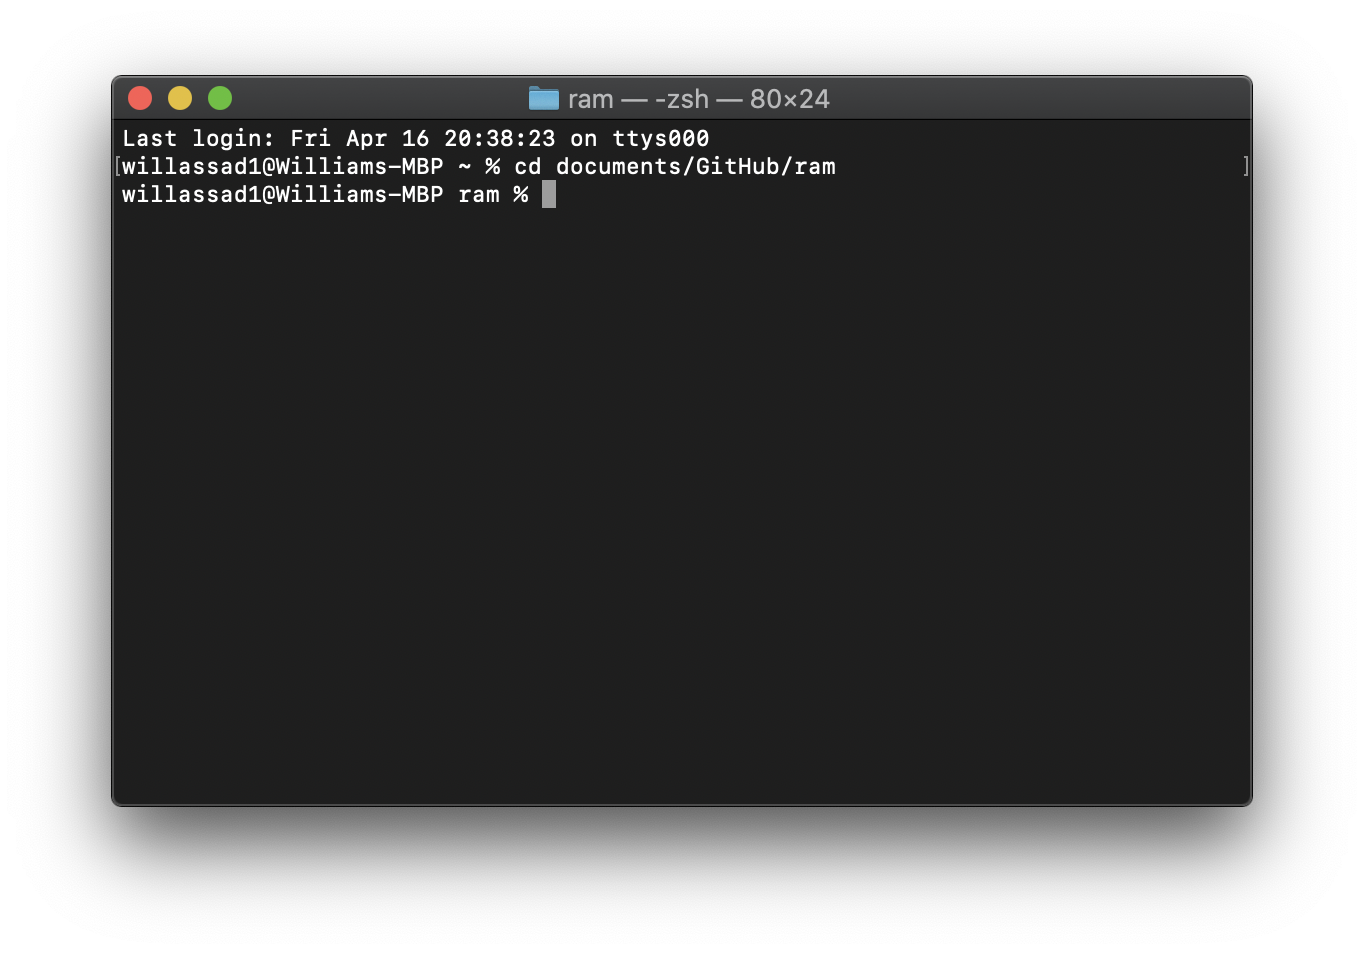
\includegraphics[scale=0.45]{terminal2.png}
        \end{center}
            
        \item Now run the command \texttt{python install.py} or \texttt{python3} \newline \texttt{install.py} (depending on version used).
            
        \begin{center}
            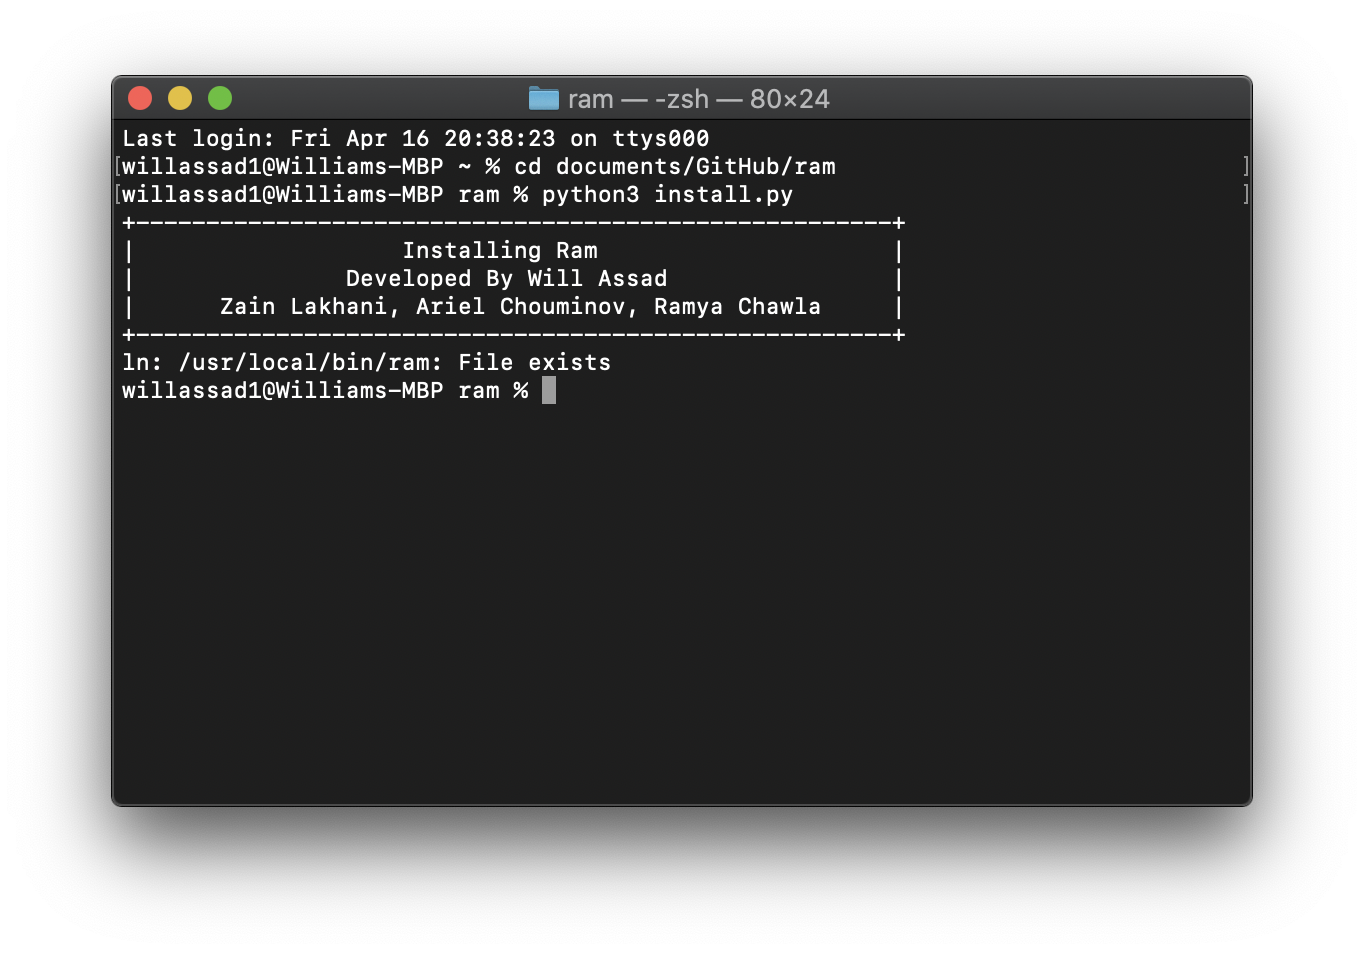
\includegraphics[scale=0.45]{terminal3.png}
        \end{center}
            
        \item You can now write a new \texttt{.ram} file in any text editor. We even defined custom syntax highlighting for \texttt{*.ram} files in PyCharm!
            
        \begin{center}
            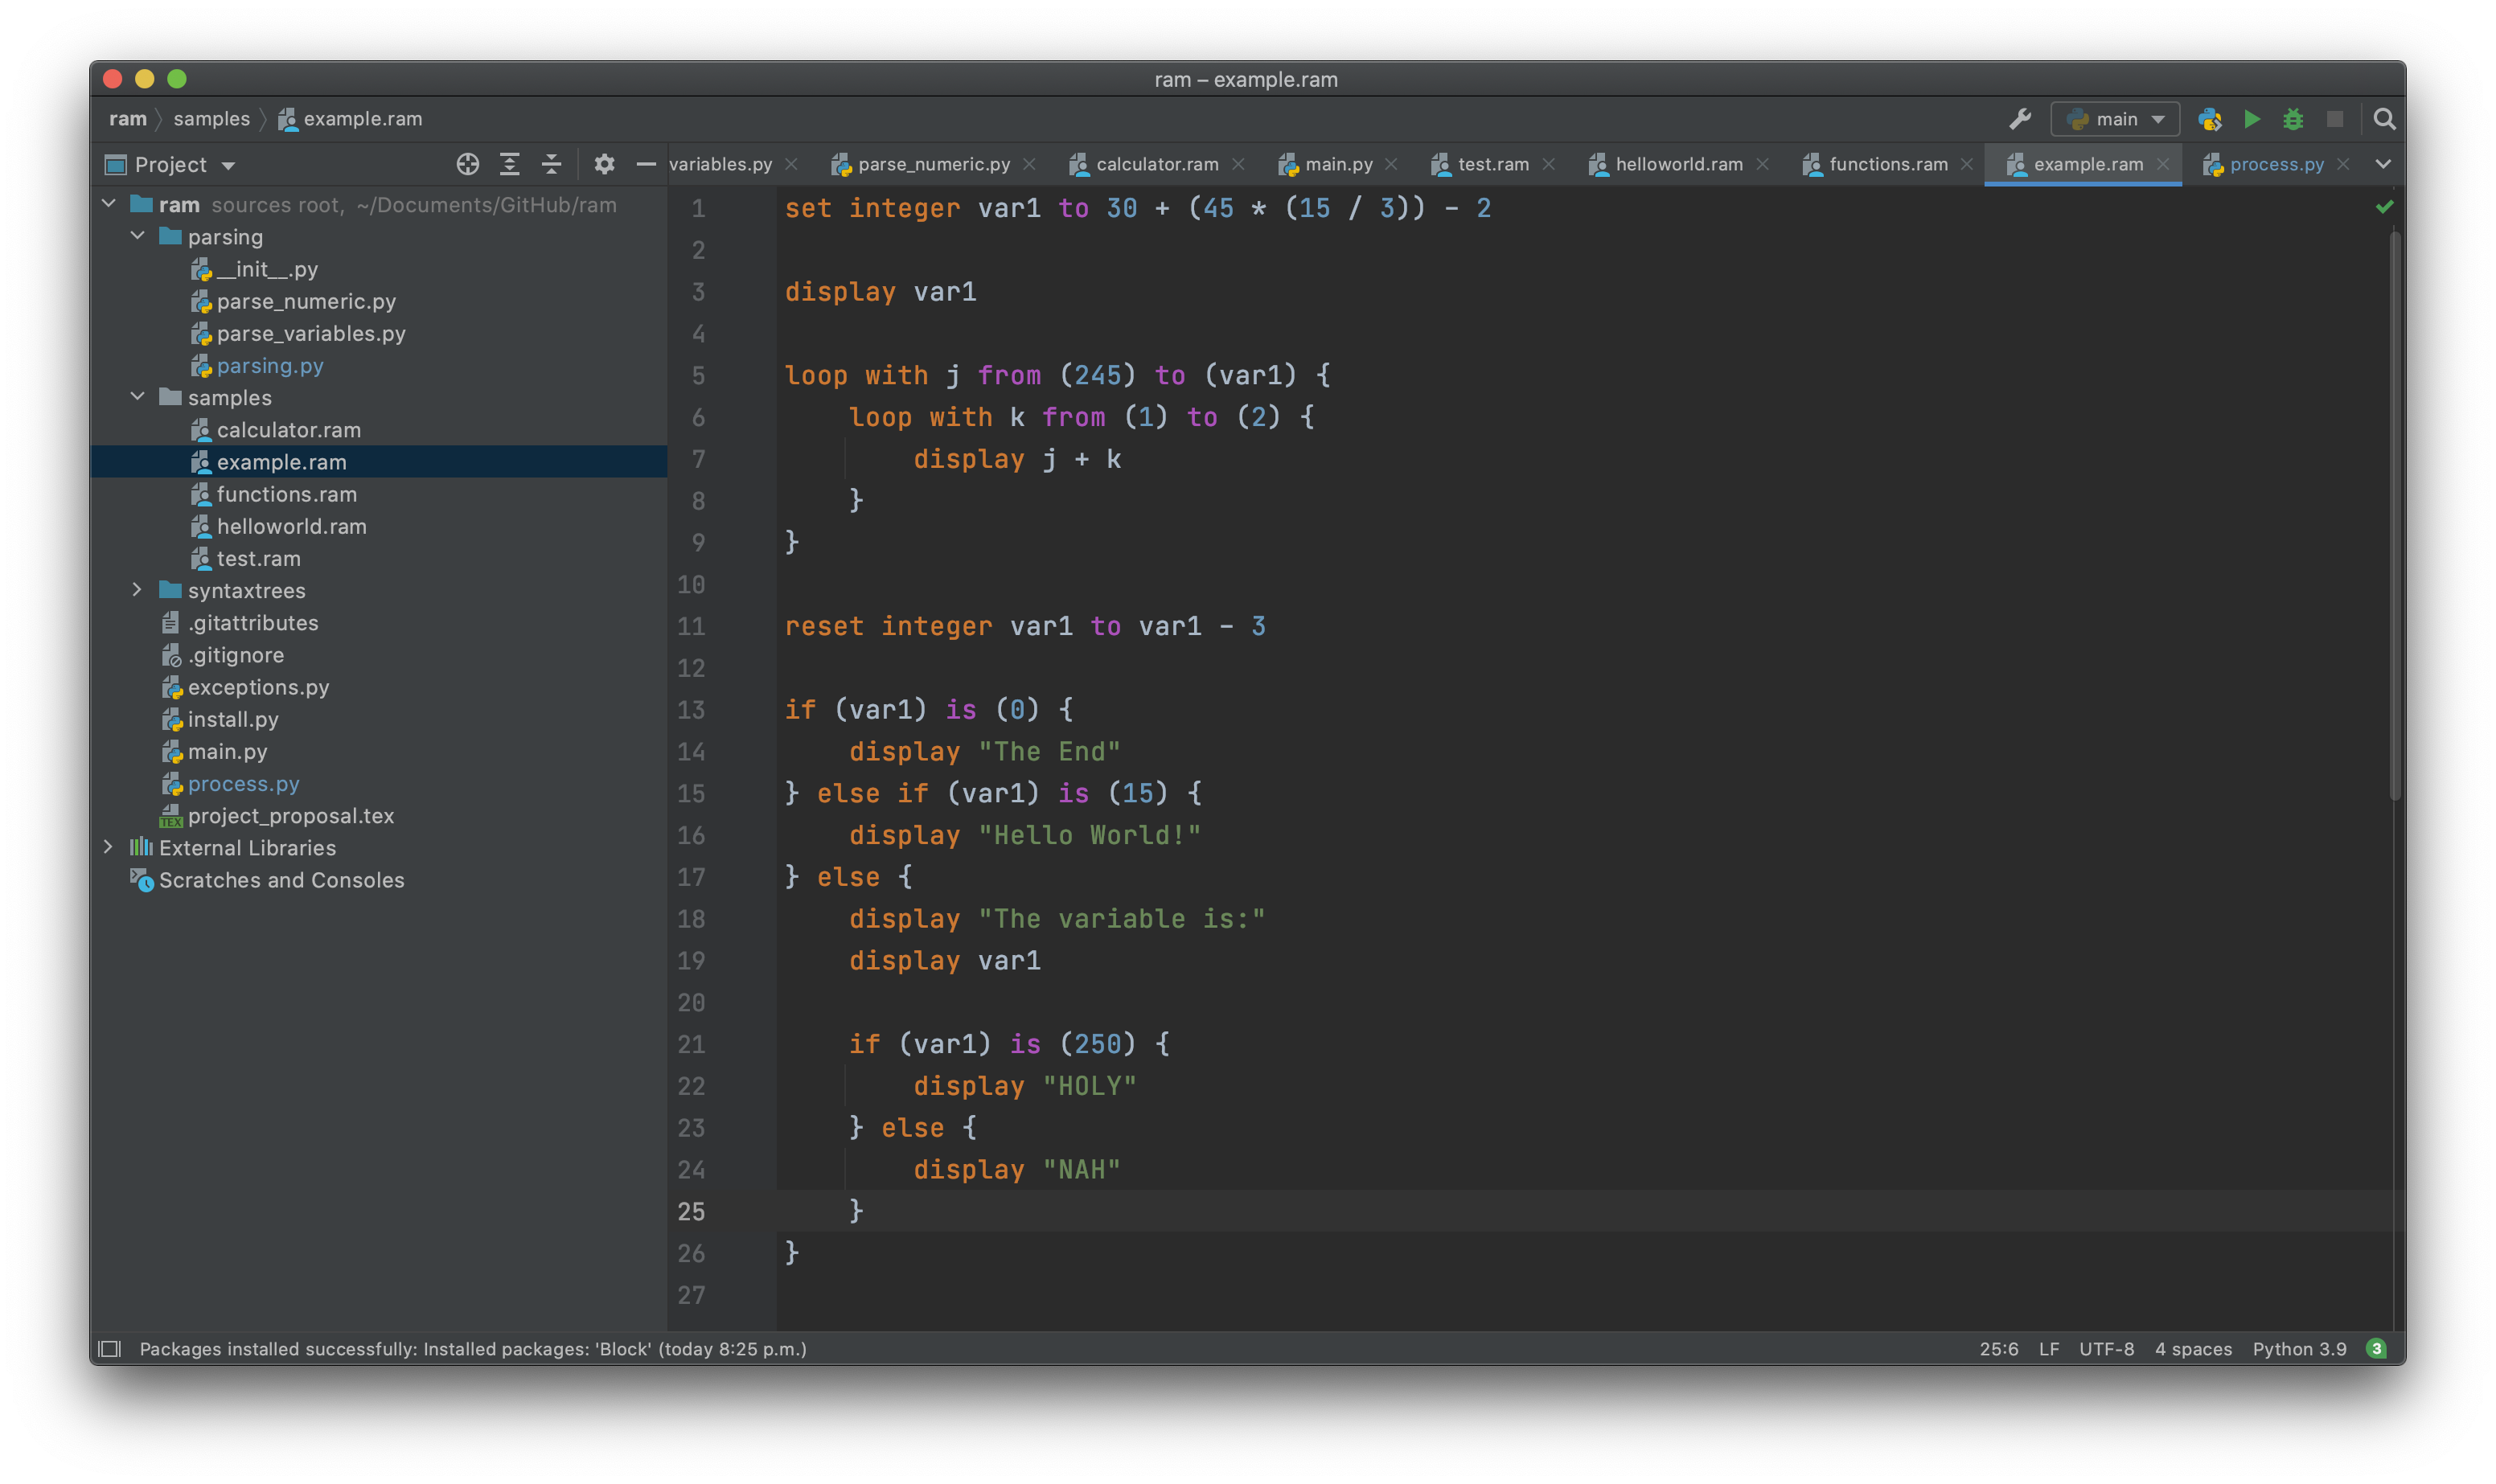
\includegraphics[scale=0.2]{terminal5.png}
        \end{center}
            
        \item Then run the file using the command \texttt{ram <filepath>.ram} or simply \texttt{ram}.
            
        \begin{center}
            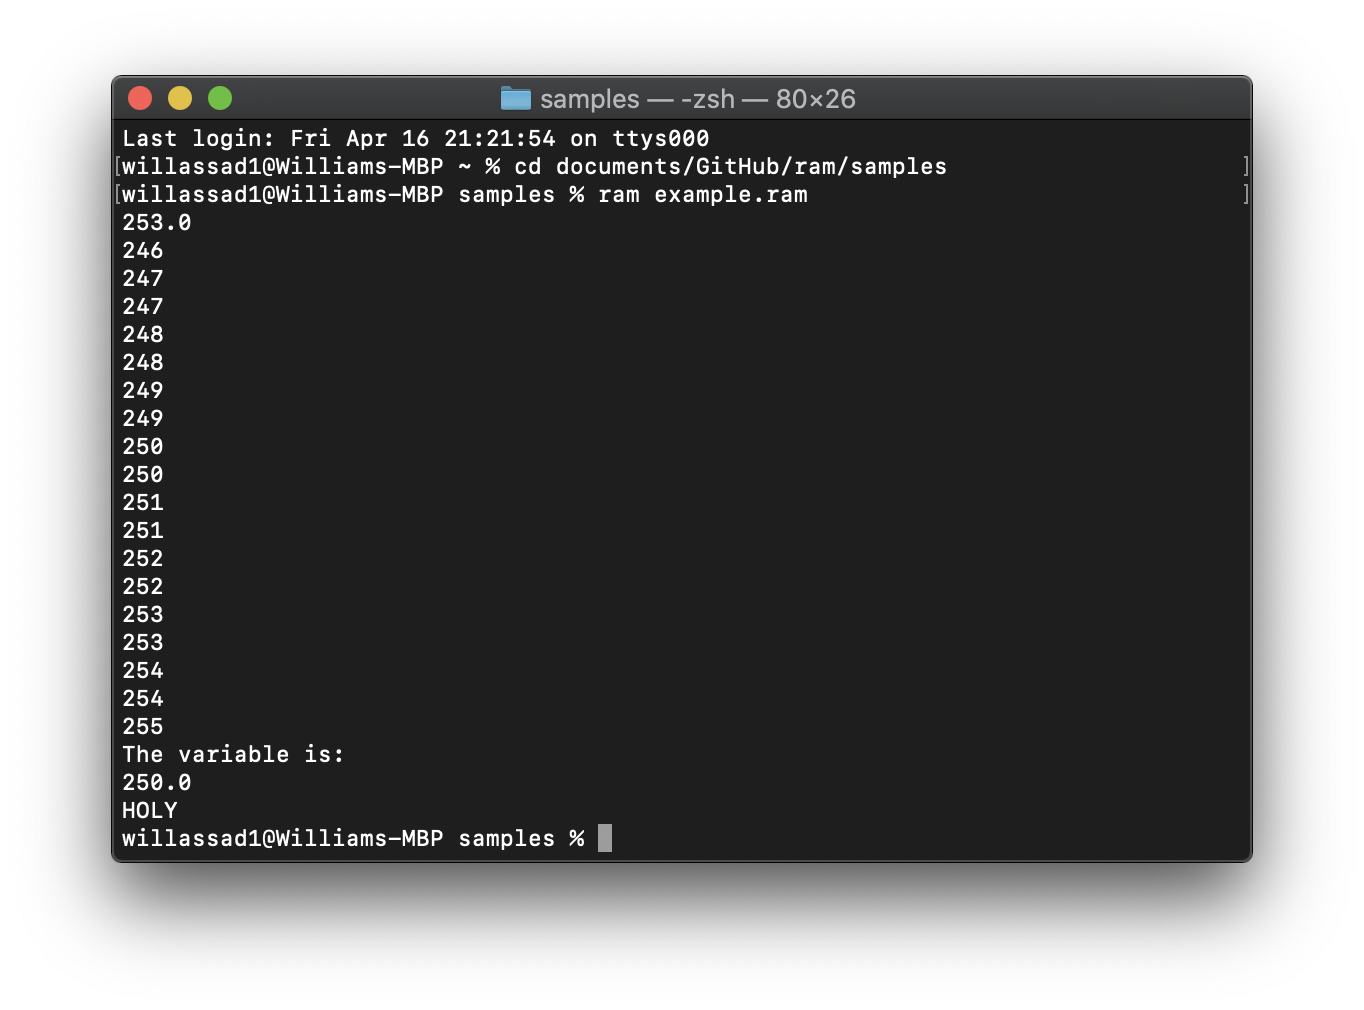
\includegraphics[scale=0.45]{terminal6.png}
        \end{center}
    \end{itemize} 

\section{Using Windows}

\emph{Note:} only python console is supported in Windows.

\subsection*{Python Console}

\begin{itemize}
        \item You can write a new \texttt{.ram} file in any text editor. We even defined custom syntax highlighting for \texttt{*.ram} files in PyCharm! 
            
        \begin{center}
            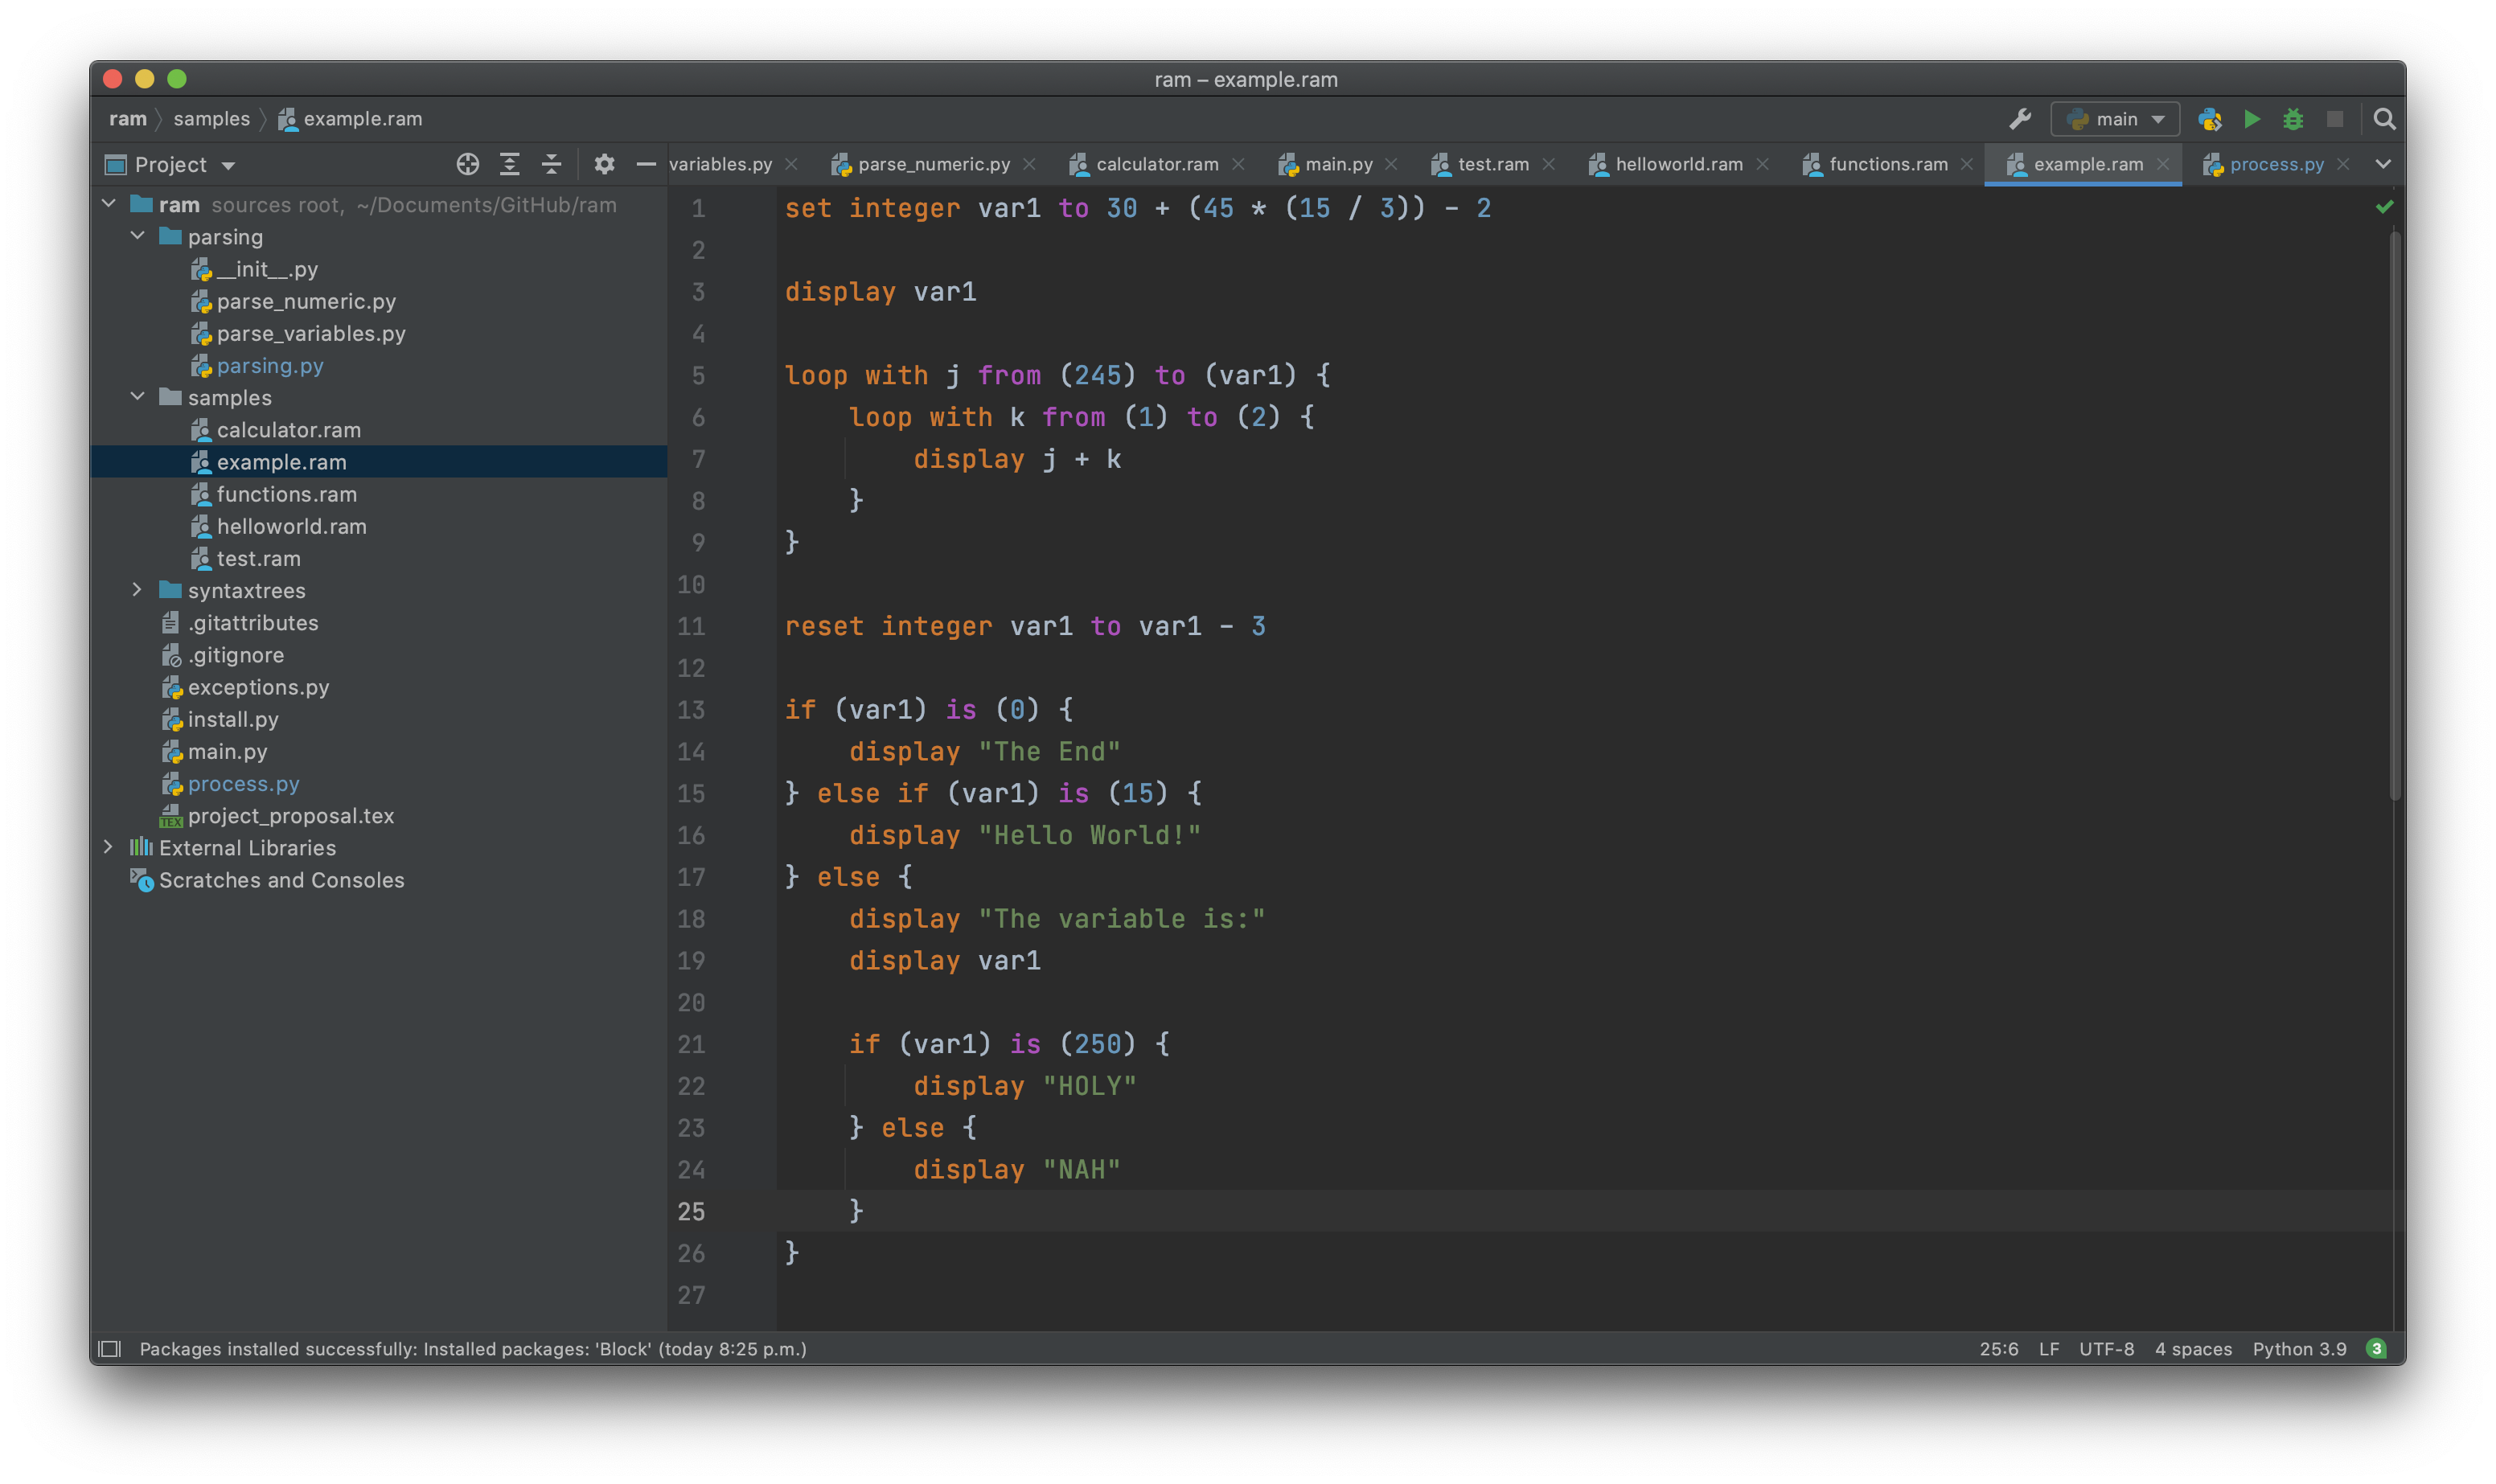
\includegraphics[scale=0.18]{terminal5.png}
        \end{center}
            
        \item Run main.py
            
        \item You will be prompted to enter the file path of the .ram file to run.
            
        \bigskip
            
        \bigskip
        
\end{itemize}


\section{Technical Notes}

\begin{itemize}
    \item Strings must be defined with double quotes, not single quotes.
    
    \item Return statements, if any, must be the last line in a function.
    
    \item There cannot be spaces when calling functions (i.e. \texttt{f[x=40,y=some\_variable]}).
    
    \item The ending curly brace of a loop, function, or if statement must be the only item in the line.
    
\end{itemize}

\end{document}